% ---------------------------------------------------------------------- 
\subsection{IPsec}
\label{section:IPSECgeneral}

% ciphersuites current 2013-12-09

\subsubsection{Settings}

\paragraph{Assumptions:}
We assume the use of IKE (v1 or v2) and ESP for this document.

\paragraph{Authentication:}
IPSEC authentication should optimally be performed via RSA signatures,
with a key size of 2048 bits or more. Configuring only the trusted CA
that issued the peer certificate provides for additional protection
against fake certificates.

If you need to use Pre-Shared Key authentication:

\begin{enumerate}
  \item Choose a \textbf{random}, \textbf{long enough} PSK (see below)
  \item Use a \textbf{separate} PSK for any IPSEC connection
  \item Change the PSKs regularly
\end{enumerate}

The size of the PSK should not be shorter than the output size of
the hash algorithm used in IKE\footnote{It is used in a HMAC, see
RFC2104~\cite{rfc2104} and the discussion starting
in \url{http://www.vpnc.org/ietf-ipsec/02.ipsec/msg00268.html}.}.

For a key composed of upper- and lowercase letters, numbers, and two
additional symbols\footnote{64 possible values = 6 bits},
table~\ref{tab:IPSEC_psk_len} gives the minimum lengths in characters.


\ctable[%
pos=ht,
caption={PSK lengths},
label=tab:IPSEC_psk_len,
]{lc}{}{
\FL    IKE Hash & PSK length (chars)
\ML    SHA256 & 43
\NN    SHA384 & 64
\NN    SHA512 & 86
\LL}

\paragraph{Cryptographic Suites:}
IPSEC Cryptographic Suites are pre-defined settings for all the items
of a configuration; they try to provide a balanced security level and
make setting up VPNs easier.
\footnote{RFC6379~\cite{rfc6379}, RFC4308~\cite{rfc4308}}

When using any of those suites, make sure to enable ``Perfect Forward
Secrecy`` for Phase 2, as this is not specified in the suites. The
equivalents to the recommended ciphers suites in section
\ref{section:recommendedciphers} are shown in
table~\ref{tab:IPSEC_suites}.

\ctable[%
caption={IPSEC Cryptographic Suites},
label=tab:IPSEC_suites,
]{>{\raggedright}p{3cm}>{\raggedright}p{3cm}l}{}{
\FL    Configuration A & Configuration B & Notes
\ML
    \texttt{Suite-B-GCM-256} &
    \texttt{Suite-B-GCM-128} \newline \texttt{VPN-B} &
    All Suite-B variants use NIST elliptic curves
\LL}
\paragraph{Phase 1:}

Alternatively to the pre-defined cipher suites, you can define your
own, as described in this and the next section.

Phase 1 is the mutual authentication and key exchange phase;
table~\ref{tab:IPSEC_ph1_params} shows the parameters.

Use only ``main mode``, as ``aggressive mode`` has known security
vulnerabilities \footnote{\url{http://ikecrack.sourceforge.net/}}.

\ctable[%
caption={IPSEC Phase 1 parameters},
label=tab:IPSEC_ph1_params,
]{lll}{}{%
\FL    & Configuration A & Configuration B
\ML    Mode & Main Mode & Main Mode
\NN    Encryption & AES-256 & AES, CAMELLIA (-256 or -128)
\NN    Hash & SHA2-* & SHA2-*, SHA1
\NN    DH Group & Group 14-18 & Group 14-18
%\NN    Lifetime & \todo{need recommendations; 1 day seems to be common practice} &
\LL}

\paragraph{Phase 2:}
Phase 2 is where the parameters that protect the actual data are negotiated; recommended
parameters are shown in table \ref{tab:IPSEC_ph2_params}.

\ctable[%
caption={IPSEC Phase 2 parameters},
label=tab:IPSEC_ph2_params,
]{l>{\raggedright}p{4.5cm}>{\raggedright}p{6cm}}{}{%
\FL    & Configuration A & Configuration B
\ML    Perfect Forward Secrecy & \yes & \yes
\NN    Encryption & %
    \mbox{AES-GCM-16}, \mbox{AES-CTR}, \mbox{AES-CCM-16}, \mbox{AES-256} &%
    \mbox{AES-GCM-16}, \mbox{AES-CTR}, \mbox{AES-CCM-16}, \mbox{AES-256}, \mbox{CAMELLIA-256}, \mbox{AES-128}, \mbox{CAMELLIA-128}
\NN    Hash & SHA2-* (or none for AEAD) & SHA2-*, SHA1 (or none for AEAD)
\NN    DH Group & Same as Phase 1 & Same as Phase 1
%\NN    Lifetime & \todo{need recommendations; 1-8 hours is common} &
\LL}

\subsubsection{References}
\begin{itemize*}
  \item ``A Cryptographic Evaluation of IPsec'', Niels Ferguson and Bruce
    Schneier: \url{https://www.schneier.com/paper-ipsec.pdf}
\end{itemize*}


%----------------------------------------------------------------------
\subsection{Check Point FireWall-1}

% Attention, only example...
%Checkpoint firewall is a \gls{firewall} that ....

\subsubsection{Tested with Versions}
\begin{itemize*}
  \item R77 (should work with any currently supported version)
\end{itemize*}

\subsubsection{Settings}
Please see section \ref{section:IPSECgeneral} for guidance on
parameter choice. In this section, we will configure a strong setup
according to ``Configuration A''.

This is based on the concept of a ``VPN Community'', which has all the
settings for the gateways that are included in that community.
Communities can be found in the ``IPSEC VPN'' tab of SmartDashboard.

\begin{figure}[p]
  \centering
  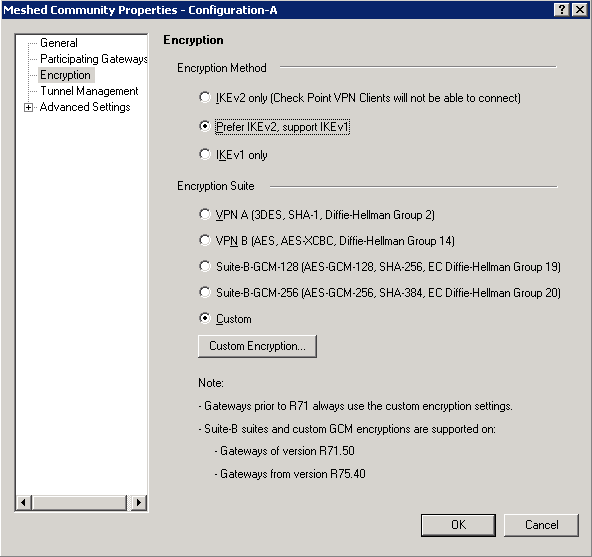
\includegraphics[width=0.592\textwidth]{img/checkpoint_1.png}
  \caption{VPN Community encryption properties}
  \label{fig:checkpoint_1}
\end{figure}

Either choose one of the encryption suites in the properties dialog
(figure \ref{fig:checkpoint_1}), or proceed to
``Custom Encryption...'', where you can set encryption and hash for
Phase 1 and 2 (figure \ref{fig:checkpoint_2}).

\begin{figure}[p]
  \centering
  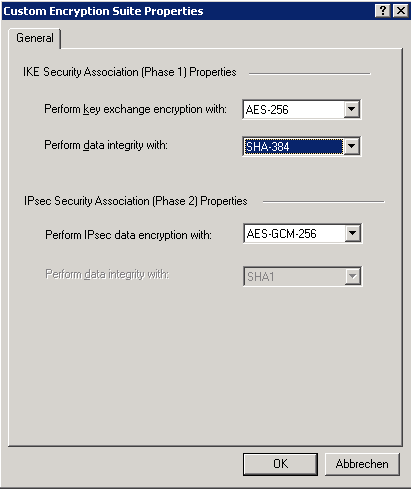
\includegraphics[width=0.411\textwidth]{img/checkpoint_2.png}
  \caption{Custom Encryption Suite Properties}
  \label{fig:checkpoint_2}
\end{figure}

The Diffie-Hellman groups and Perfect Forward Secrecy Settings can be
found under ``Advanced Settings'' / ``Advanced VPN Properties''
(figure \ref{fig:checkpoint_3}).

\begin{figure}[p]
  \centering
  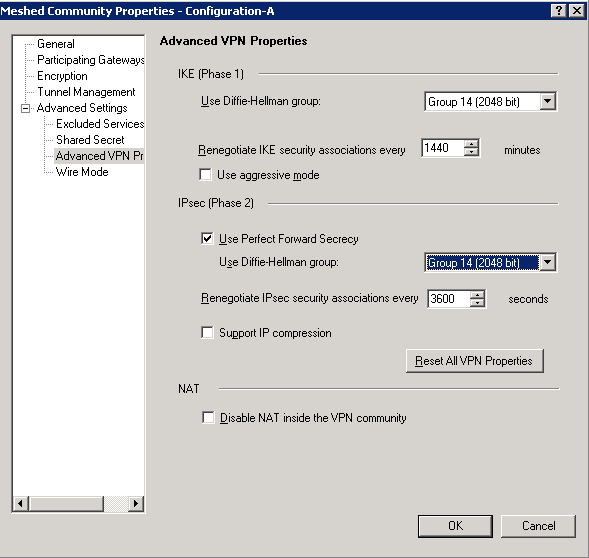
\includegraphics[width=0.589\textwidth]{img/checkpoint_3.png}
  \caption{Advanced VPN Properties}
  \label{fig:checkpoint_3}
\end{figure}


\subsubsection{Additional settings}
For remote Dynamic IP Gateways, the settings are not taken from the
community, but set in the ``Global Properties'' dialog under ``Remote
Access'' / ``VPN Authentication and Encryption''. Via the ``Edit...''
button, you can configure sets of algorithms that all gateways support
(figure \ref{fig:checkpoint_4}).

\begin{figure}[p]
  \centering
  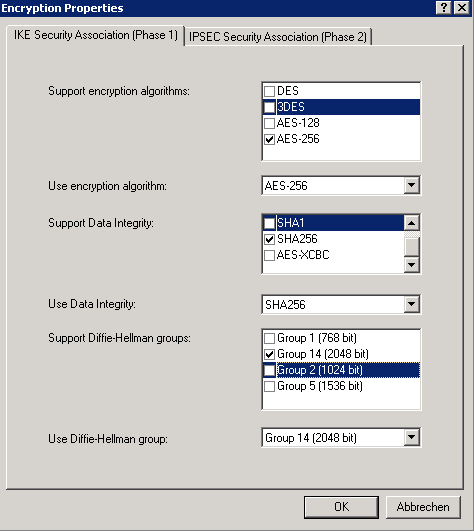
\includegraphics[width=0.474\textwidth]{img/checkpoint_4.png}
  \caption{Remote Access Encryption Properties}
  \label{fig:checkpoint_4}
\end{figure}

Please note that these settings restrict the available algorithms for
\textbf{all} gateways, and also influence the VPN client connections.

%\subsubsection{Justification for special settings (if needed)}

%\subsubsection{Limitations}

\subsubsection{References}
\begin{itemize*}
  \item Check Point \href{https://sc1.checkpoint.com/documents/R77/CP_R77_VPN_AdminGuide/html_frameset.htm}{VPN R77 Administration Guide} (may require a UserCenter account to access)
\end{itemize*}

%\subsubsection{How to test}

%% cipherstrings current 2013-12-09
% ---------------------------------------------------------------------- 
\FloatBarrier % the preceding section has several figures. Floating them too far away might get confusing for readers.

\subsection{OpenVPN}

\subsubsection{Tested with Versions}
\begin{itemize*}
  \item OpenVPN 2.3.10 from Ubuntu Xenial 16.04.1 LTS linked against openssl (libssl.so.1.0.0)
  \item OpenVPN 2.3.2 from Debian ``wheezy-backports'' linked against openssl (libssl.so.1.0.0)
  \item OpenVPN 2.2.1 from Debian Wheezy linked against openssl (libssl.so.1.0.0)
  \item OpenVPN 2.3.2 for Windows
\end{itemize*}

\subsubsection{Settings}

\paragraph{General}
We describe a configuration with certificate-based authentication; see
below for details on the \verb|easyrsa| tool to help you with that.

OpenVPN uses TLS only for authentication and key exchange. The
bulk traffic is then encrypted and authenticated with the OpenVPN
protocol using those keys.

Note that while the \verb|tls-cipher| option takes a list of ciphers
that is then negotiated as usual with TLS, the \verb|cipher|
and \verb|auth| options both take a single argument that must match on
client and server.

OpenVPN duplexes the tunnel into a data and a control channel. The control
channel is a usual TLS connection, the data channel currently uses 
encrypt-then-mac CBC, see \url{https://github.com/BetterCrypto/Applied-Crypto-Hardening/pull/91#issuecomment-75365286}


\paragraph{Server Configuration}
~\\
% the cipherlist here is config B without the ECDHE strings, because
% it must fit in 256 bytes...
% DO NOT CHANGE TO THE CIPHERSTRING MACRO!
\configfile{server.conf}{248-250}{Cipher configuration for OpenVPN (Server)}

\paragraph{Client Configuration}
Client and server have to use compatible configurations, otherwise they can't communicate.
The \verb|cipher| and \verb|auth| directives have to be identical.

% the cipherlist here is config B without the ECDHE strings, because
% it must fit in 256 bytes...
% DO NOT CHANGE TO THE CIPHERSTRING MACRO!
\configfile{client.conf}{44-45,115-121}{Cipher and TLS configuration for OpenVPN (Server)}

\subsubsection{Justification for special settings}
OpenVPN 2.3.1 changed the values that the \verb|tls-cipher| option
expects from OpenSSL to IANA cipher names. That means from that
version on you will get ``Deprecated TLS cipher name'' warnings for
the configurations above. You cannot use the selection strings from
section \ref{section:recommendedciphers} directly from 2.3.1 on, which
is why we give an explicit cipher list here.

In addition, there is a 256 character limit on configuration file line
lengths; that limits the size of cipher suites, so we dropped all
ECDHE suites.

The configuration shown above is compatible with all tested versions.


\subsubsection{References}
\begin{itemize*}
  \item OpenVPN Documentation: \emph{Security Overview} \url{https://openvpn.net/index.php/open-source/documentation/security-overview.html}
\end{itemize*}

%\subsubsection{How to test}


\subsubsection{Additional settings}

\paragraph{Key renegotiation interval}
The default for renegotiation of encryption keys is one hour
(\verb|reneg-sec 3600|). If you
transfer huge amounts of data over your tunnel, you might consider
configuring a shorter interval, or switch to a byte- or packet-based
interval (\verb|reneg-bytes| or \verb|reneg-pkts|).

\paragraph{Insecure ciphers}

Sweet32\footnote{\url{https://sweet32.info/}} is an attack on 64-bit block
ciphers, such as \verb|3DES| and \verb|Blowfish| in OpenVPN. The following
ciphers are affected, and should no longer be used:
\begin{itemize*}
  \item BF-*
  \item DES* (including 3DES variants)
  \item RC2-*
\end{itemize*}
The following ciphers are not affected:
\begin{itemize*}
  \item AES-*
  \item CAMELLIA-*
  \item SEED-*
\end{itemize*}
According to mitigation section on Sweet32 website\footnote{\url{https://sweet32.info/\#impact}}
users users should change the cipher from the DES or Blowfish to AES
(\verb|cipher AES-128-CBC|). If cipher change is not possible users can
mitigate the attack by forcing frequent rekeying (\verb|reneg-bytes 64000000|).

\paragraph{Fixing ``easy-rsa''}
When installing an OpenVPN server instance, you are probably using
\emph{easy-rsa} to generate keys and certificates.
The file \verb|vars| in the easyrsa installation directory has a
number of settings that should be changed to secure values:

\configfile{vars}{53-53,56-56,59-59}{Sane default values for OpenVPN (easy-rsa)}


This will enhance the security of the key generation by using RSA keys
with a length of 4096 bits, and set a lifetime of one year for the
server/client certificates and five years for the CA certificate. \textbf{NOTE: 4096 bits is only an example of how to do this with easy-rsa.} See also section \ref{section:keylengths} for a discussion on keylengths.

In addition, edit the \verb|pkitool| script and replace all occurrences
of \verb|sha1| with \verb|sha256|, to sign the certificates with
SHA256.

\subsubsection{Limitations}
Note that the ciphersuites shown by \verb|openvpn --show-tls| are \emph{known}, but not necessarily \emph{supported} \footnote{\url{https://community.openvpn.net/openvpn/ticket/304}}.

Which cipher suite is actually used can be seen in the logs:

\verb|Control Channel: TLSv1, cipher TLSv1/SSLv3 DHE-RSA-CAMELLIA256-SHA, 2048 bit RSA|


% ---------------------------------------------------------------------- 
\subsection{PPTP}

PPTP is considered insecure, Microsoft recommends to ``use a more secure VPN
tunnel''\footnote{\url{http://technet.microsoft.com/en-us/security/advisory/2743314}}.

There is a cloud service that cracks the underlying MS-CHAPv2
authentication protocol for the price of USD~200\footnote{\url{https://www.cloudcracker.com/blog/2012/07/29/cracking-ms-chap-v2/}},
and given the resulting MD4 hash, all PPTP traffic for a user can
be decrypted.

% ---------------------------------------------------------------------- 
\subsection{Cisco ASA}
The following settings reflect our recommendations as best as possible on the Cisco ASA platform. These are - of course - just settings regarding SSL/TLS (i.e. Cisco AnyConnect) and IPsec. For further security settings regarding this platform the appropriate Cisco guides should be followed.


\subsubsection{Tested with Versions}
\begin{itemize*}
  \item 9.8(2)38 - X-series model
\end{itemize*}

\subsubsection{Settings}
\begin{lstlisting}
crypto ipsec ikev2 ipsec-proposal AES-Fallback
 protocol esp encryption aes-256 aes-192 aes
 protocol esp integrity sha-512 sha-384 sha-256
crypto ipsec ikev2 ipsec-proposal AES-GCM-Fallback
 protocol esp encryption aes-gcm-256 aes-gcm-192 aes-gcm
 protocol esp integrity sha-512 sha-384 sha-256
crypto ipsec ikev2 ipsec-proposal AES128-GCM
 protocol esp encryption aes-gcm
 protocol esp integrity sha-512
crypto ipsec ikev2 ipsec-proposal AES192-GCM
 protocol esp encryption aes-gcm-192
 protocol esp integrity sha-512
crypto ipsec ikev2 ipsec-proposal AES256-GCM
 protocol esp encryption aes-gcm-256
 protocol esp integrity sha-512
crypto ipsec ikev2 ipsec-proposal AES
 protocol esp encryption aes
 protocol esp integrity sha-1 md5
crypto ipsec ikev2 ipsec-proposal AES192
 protocol esp encryption aes-192
 protocol esp integrity sha-1 md5
crypto ipsec ikev2 ipsec-proposal AES256
 protocol esp encryption aes-256
 protocol esp integrity sha-1 md5
crypto ipsec ikev2 sa-strength-enforcement
crypto ipsec security-association pmtu-aging infinite
crypto dynamic-map SYSTEM_DEFAULT_CRYPTO_MAP 65535 set pfs group14
crypto dynamic-map SYSTEM_DEFAULT_CRYPTO_MAP 65535 set ikev2 ipsec-proposal AES256-GCM AES192-GCM AES128-GCM AES-GCM-Fallback AES-Fallback
crypto map Outside-DMZ_map 65535 ipsec-isakmp dynamic SYSTEM_DEFAULT_CRYPTO_MAP
crypto map Outside-DMZ_map interface Outside-DMZ

crypto ikev2 policy 1
 encryption aes-gcm-256
 integrity null
 group 14
 prf sha512 sha384 sha256 sha
 lifetime seconds 86400
crypto ikev2 policy 2
 encryption aes-gcm-256 aes-gcm-192 aes-gcm
 integrity null
 group 14
 prf sha512 sha384 sha256 sha
 lifetime seconds 86400
crypto ikev2 policy 3
 encryption aes-256 aes-192 aes
 integrity sha512 sha384 sha256
 group 14
 prf sha512 sha384 sha256 sha
 lifetime seconds 86400
crypto ikev2 policy 4
 encryption aes-256 aes-192 aes
 integrity sha512 sha384 sha256 sha
 group 14
 prf sha512 sha384 sha256 sha
 lifetime seconds 86400
crypto ikev2 enable Outside-DMZ client-services port 443
crypto ikev2 remote-access trustpoint ASDM_TrustPoint0

ssl client-version tlvs1
ssl server-version tlsv1
ssl cipher default fips
ssl cipher tlsv1 fips
ssl cipher tlsv1.1 fips
ssl cipher tlsv1.2 high
ssl cipher dtlsv1 fips
ssl dh-group group24
ssl trust-point ASDM_TrustPoint0 Outside-DMZ
\end{lstlisting}

\subsubsection{Justification for special settings}
New IPsec policies have been defined which do not make use of ciphers that may be cause for concern. Policies have a "Fallback" option to support legacy devices.

3DES has been completely disabled as such Windows XP AnyConnect Clients will no longer be able to connect.

The Cisco ASA platform does not currently support RSA Keys above 2048bits.

Legacy ASA models (e.g. 5505, 5510, 5520, 5540, 5550) do not offer the possibility to configure for SHA256/SHA384/SHA512 nor AES-GCM for IKEv2 proposals.

\subsubsection{References}
\begin{itemize*}
  \item \url{http://www.cisco.com/en/US/docs/security/asa/roadmap/asaroadmap.html}
  \item \url{http://www.cisco.com/web/about/security/intelligence/nextgen_crypto.html}
  \itme \url{https://www.cisco.com/c/en/us/td/docs/security/asa/asa98/configuration/vpn/asa-98-vpn-config/vpn-params.html}
\end{itemize*}

% add any further references or best practice documents here

%%\subsubsection{How to test}
% describe here or point the admin to tools (can be a simple footnote or \ref{} to  the tools section) which help the admin to test his settings.


% ---------------------------------------------------------------------- 
\subsection{Openswan}


\subsubsection{Tested with Version}
\begin{itemize*}
  \item Openswan 2.6.39 (Gentoo)
\end{itemize*}

\subsubsection{Settings}
Note: the available algorithms depend on your kernel configuration (when using protostack=netkey) and/or build-time options.

To list the supported algorithms
\begin{lstlisting}
$ ipsec auto --status | less
\end{lstlisting}
and look for 'algorithm ESP/IKE' at the beginning.

\begin{lstlisting}
aggrmode=no
# ike format: cipher-hash;dhgroup
# recommended ciphers:
# - aes
# recommended hashes:
# - sha2_256 with at least 43 byte PSK
# - sha2_512 with at least 86 byte PSK
# recommended dhgroups:
# - modp2048 = DH14
# - modp3072 = DH15
# - modp4096 = DH16
# - modp6144 = DH17
# - modp8192 = DH18
ike=aes-sha2_256;modp2048
type=tunnel
phase2=esp
# esp format: cipher-hash;dhgroup
# recommended ciphers configuration A:
# - aes_gcm_c-256 = AES_GCM_16
# - aes_ctr-256
# - aes_ccm_c-256 = AES_CCM_16
# - aes-256 
# additional ciphers configuration B:
# - camellia-256
# - aes-128
# - camellia-128
# recommended hashes configuration A:
# - sha2-256
# - sha2-384
# - sha2-512
# - null (only with GCM/CCM ciphers)
# additional hashes configuration B:
# - sha1
# recommended dhgroups: same as above
phase2alg=aes_gcm_c-256-sha2_256;modp2048
salifetime=8h
pfs=yes
auto=ignore
\end{lstlisting}

\subsubsection{How to test}
Start the vpn and using
\begin{lstlisting}
$ ipsec auto --status | less
\end{lstlisting}
and look for 'IKE algorithms wanted/found' and 'ESP algorithms wanted/loaded'.

\subsubsection{References}
%\todo{more specific References??}
\begin{itemize*}
  \item \url{https://www.openswan.org/}
\end{itemize*}


\subsection{tinc}
\subsubsection{Tested with Version}
\begin{itemize*}
  \item tinc 1.0.23 from Gentoo linked against OpenSSL 1.0.1e
  \item tinc 1.0.23 from Sabayon linked against OpenSSL 1.0.1e
\end{itemize*}

\paragraph*{Defaults}\mbox{}\\
tinc uses 2048 bit RSA keys, Blowfish-CBC, and SHA1 as default settings and suggests the usage of CBC mode ciphers.
Any key length up to 8192 is supported and it does not need to be a power of two. OpenSSL Ciphers and Digests are supported by tinc.

\paragraph*{Settings}\mbox{}\\
Generate keys with
\begin{lstlisting}[breaklines]
tincd -n NETNAME -K8192
\end{lstlisting}
Old keys will not be deleted (but disabled), you have to delete them manually. Add the following lines to your tinc.conf on all machines
\configfile{tinc.conf}{3-4}{Cipher and digest selection in tinc}

\paragraph*{References}\mbox{}\\
\begin{itemize}
\item tincd(8) man page
\item tinc.conf(5) man page
\item \href{http://www.tinc-vpn.org/pipermail/tinc/2014-January/003538.html}{tinc mailinglist: http://www.tinc-vpn.org/pipermail/tinc/2014-January/003538.html}
\end{itemize}


% ---------------------------------------------------------------------- 
%%\subsection{Juniper VPN}
%%\todo{write this subsubsection. AK: ask Hannes}




% ---------------------------------------------------------------------- 
%\subsection{L2TP over IPSec}
%\todo{write this subsubsection}




% ---------------------------------------------------------------------- 
%\subsection{Racoon}
%\todo{write this subsubsection}


